\documentclass[12pt]{article}
\usepackage[a4paper,bindingoffset=0.2in,
            left=1in,right=1in,top=1in,bottom=1in,
            footskip=.25in]{geometry}
\usepackage{graphicx}
\usepackage{parskip}
\usepackage{titling}

\graphicspath{ {images/} }

\title{Technical Specification}
\author{SDP Group 15-H}

\begin{document}

\begin{figure}
    \vspace*{-3em}
    \centering
    
\includegraphics[scale=.18]{logo.png}
\end{figure}

\setlength{\droptitle}{-4em}
\maketitle

\section{System Architecture}

The earliest prototype simply had four regular wheels as seen in Figure
\ref{fig:robot0}. This made us realise that we have to keep in mind the space
constraints when building the base as we need to accommodate not only the motors
for the wheels but also the kicking and grabbing mechanism.
The next more sophisticated design was a robot with four powerful kickers
that used elastics as seen in Figure \ref{fig:robot3}. This design had a
disadvantage because it was not be able to kick the ball for varying distances,
which was an essential requirement for the first milestone. Moreover, the
dimensions of the robot were exceeding the maximum size limits. Thus, a similar
design was agreed upon as seen in Figures \ref{fig:robot1} and \ref{fig:robot2}.
Advantage of this design is that it is simple and at the same time the robot can
still move fast enough to play football and the power of the kicks can be
precisely controlled.

\begin{figure}[h]
	\centering
	\begin{minipage}[b]{.48\textwidth}
        \centering
		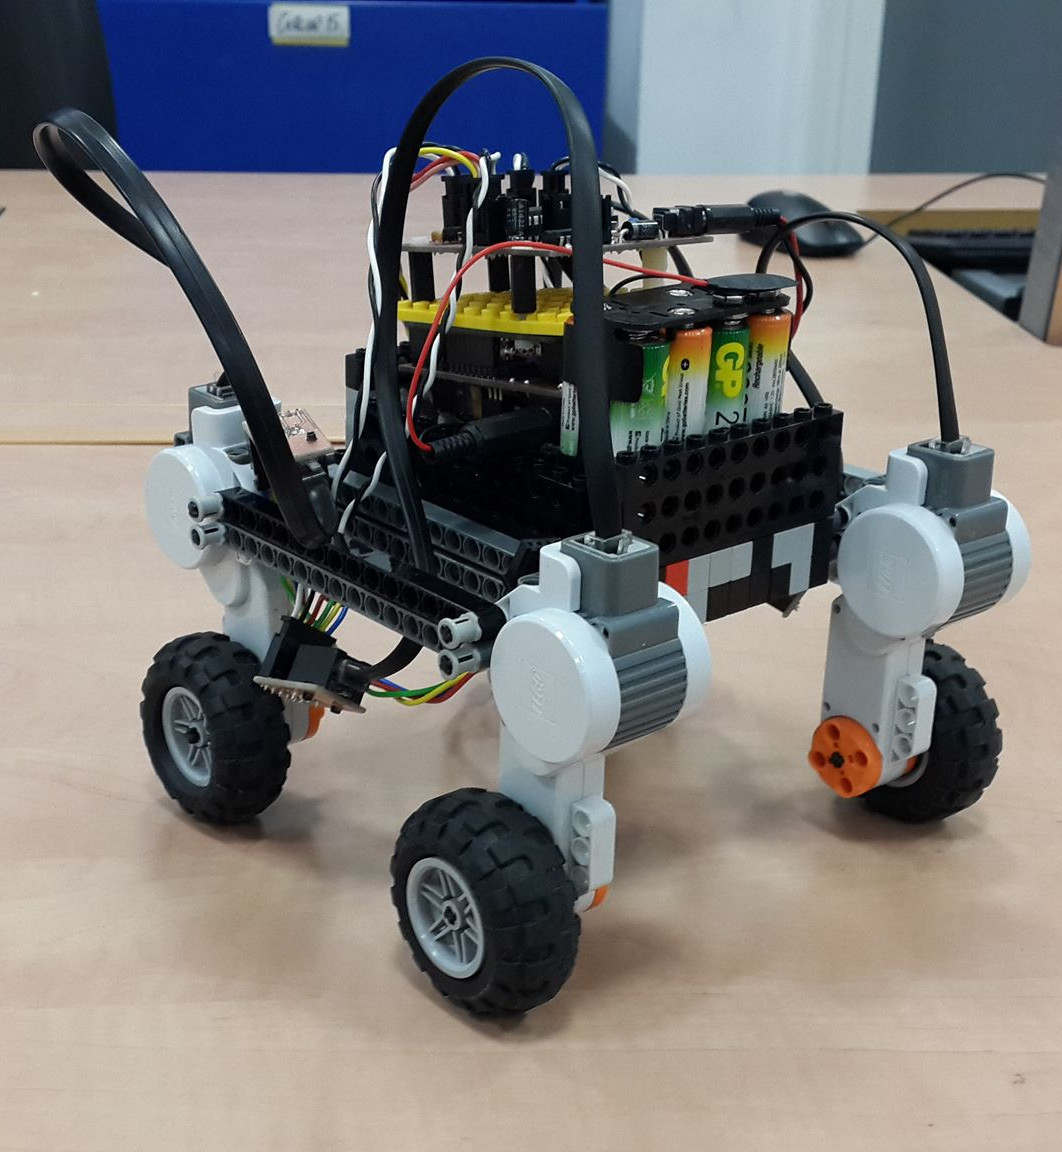
\includegraphics[scale=.18]{robot0.jpg}
		\caption{The first prototype}
		\label{fig:robot0}
	\end{minipage}
	~
	\begin{minipage}[b]{.48\textwidth}
        \centering
		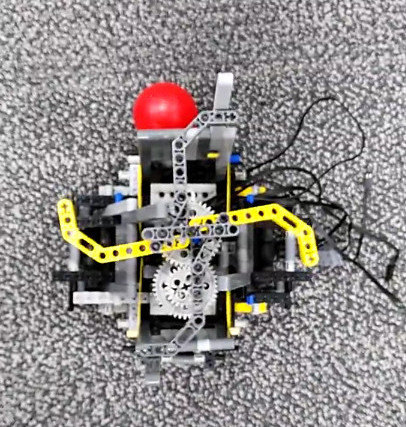
\includegraphics[scale=.65]{robot3.jpg}
		\caption{The robot with four kickers}
		\label{fig:robot3}
	\end{minipage}
\end{figure}

The grabbing mechanism of the latest design went through two iterations of
development.
The first grabber in Figure \ref{fig:robot1} was deemed not suitable because of
the obstruction of the ball which is not allowed by the football game rules.
This is related to the fact that this design had difficulties at placing the
ball in front of the kicker at initial kicking position, instead it pushed it
too far inside the kicker. It was replaced by the newest grabber design
depicted in Figure \ref{fig:robot2} which has two symmetrical grabbers that
interlock when the robot is moving to conserve space and are able to reach a
more distant ball.

\begin{figure}
	\centering
	\begin{minipage}[b]{.48\textwidth}
        \centering
		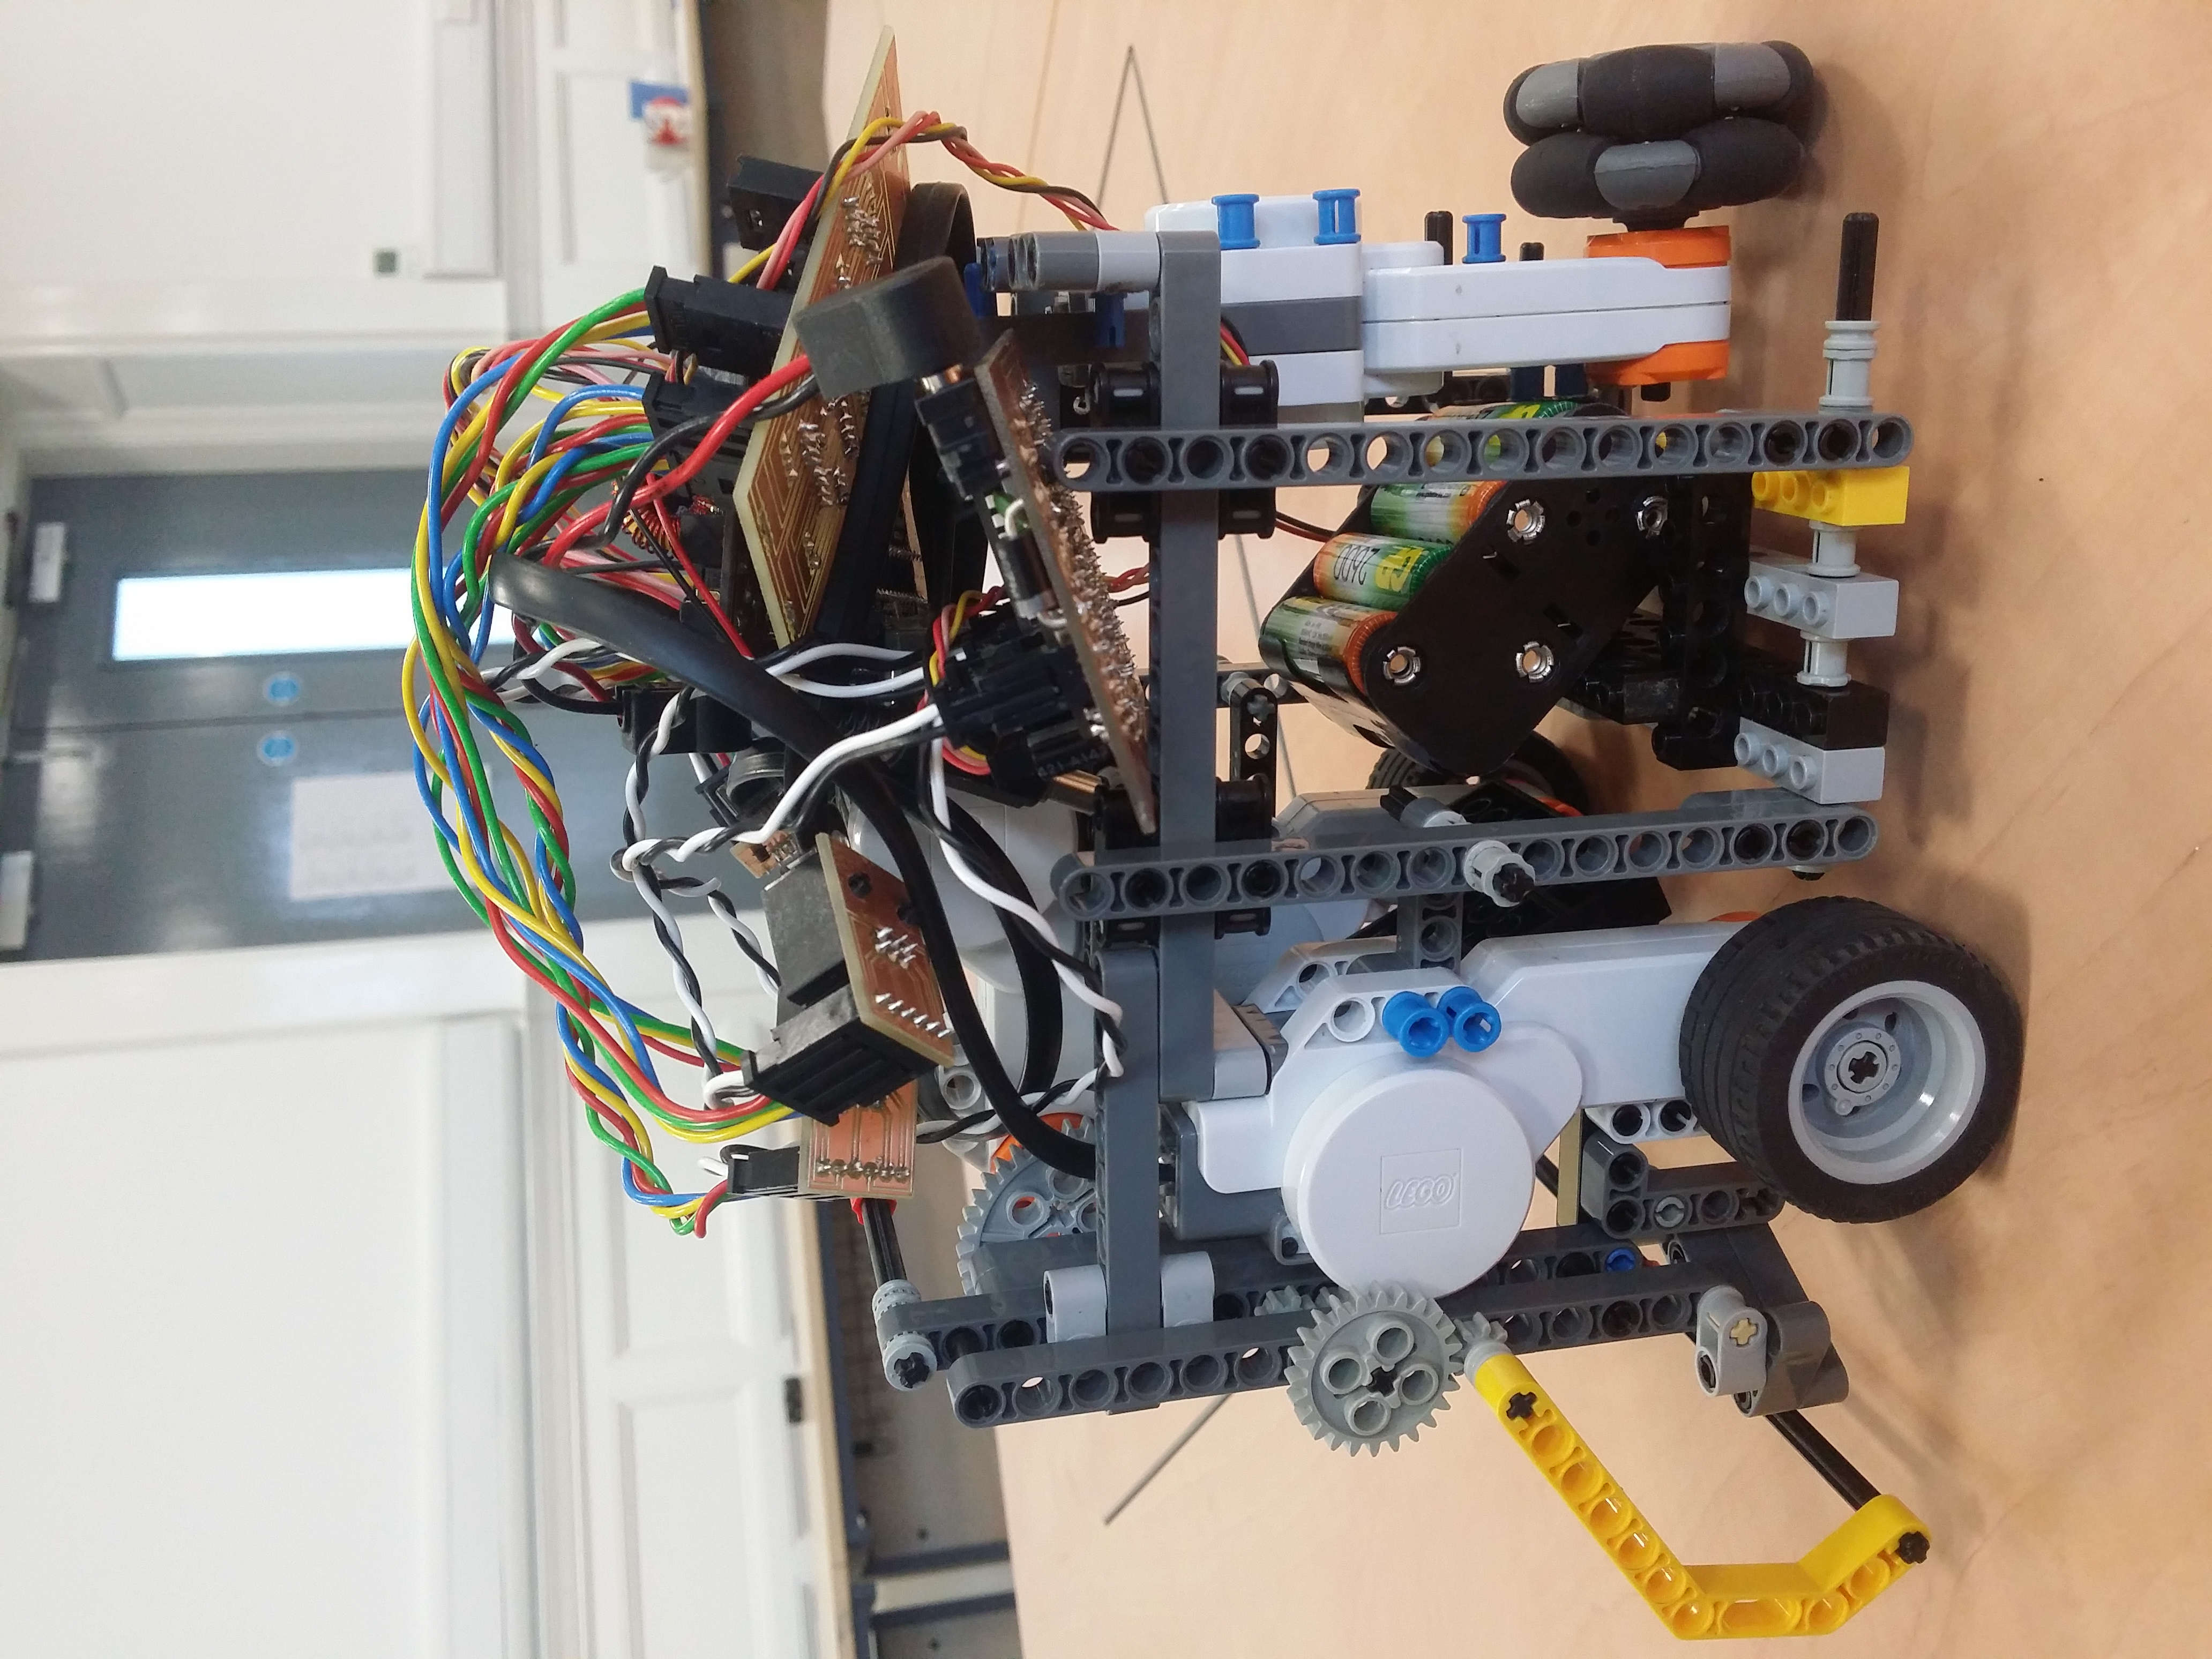
\includegraphics[scale=.065,angle=-90]{robot1.jpg}
		\caption{The third robot with the initial grabber}
		\label{fig:robot1}
	\end{minipage}
	~
	\begin{minipage}[b]{.48\textwidth}
        \centering
		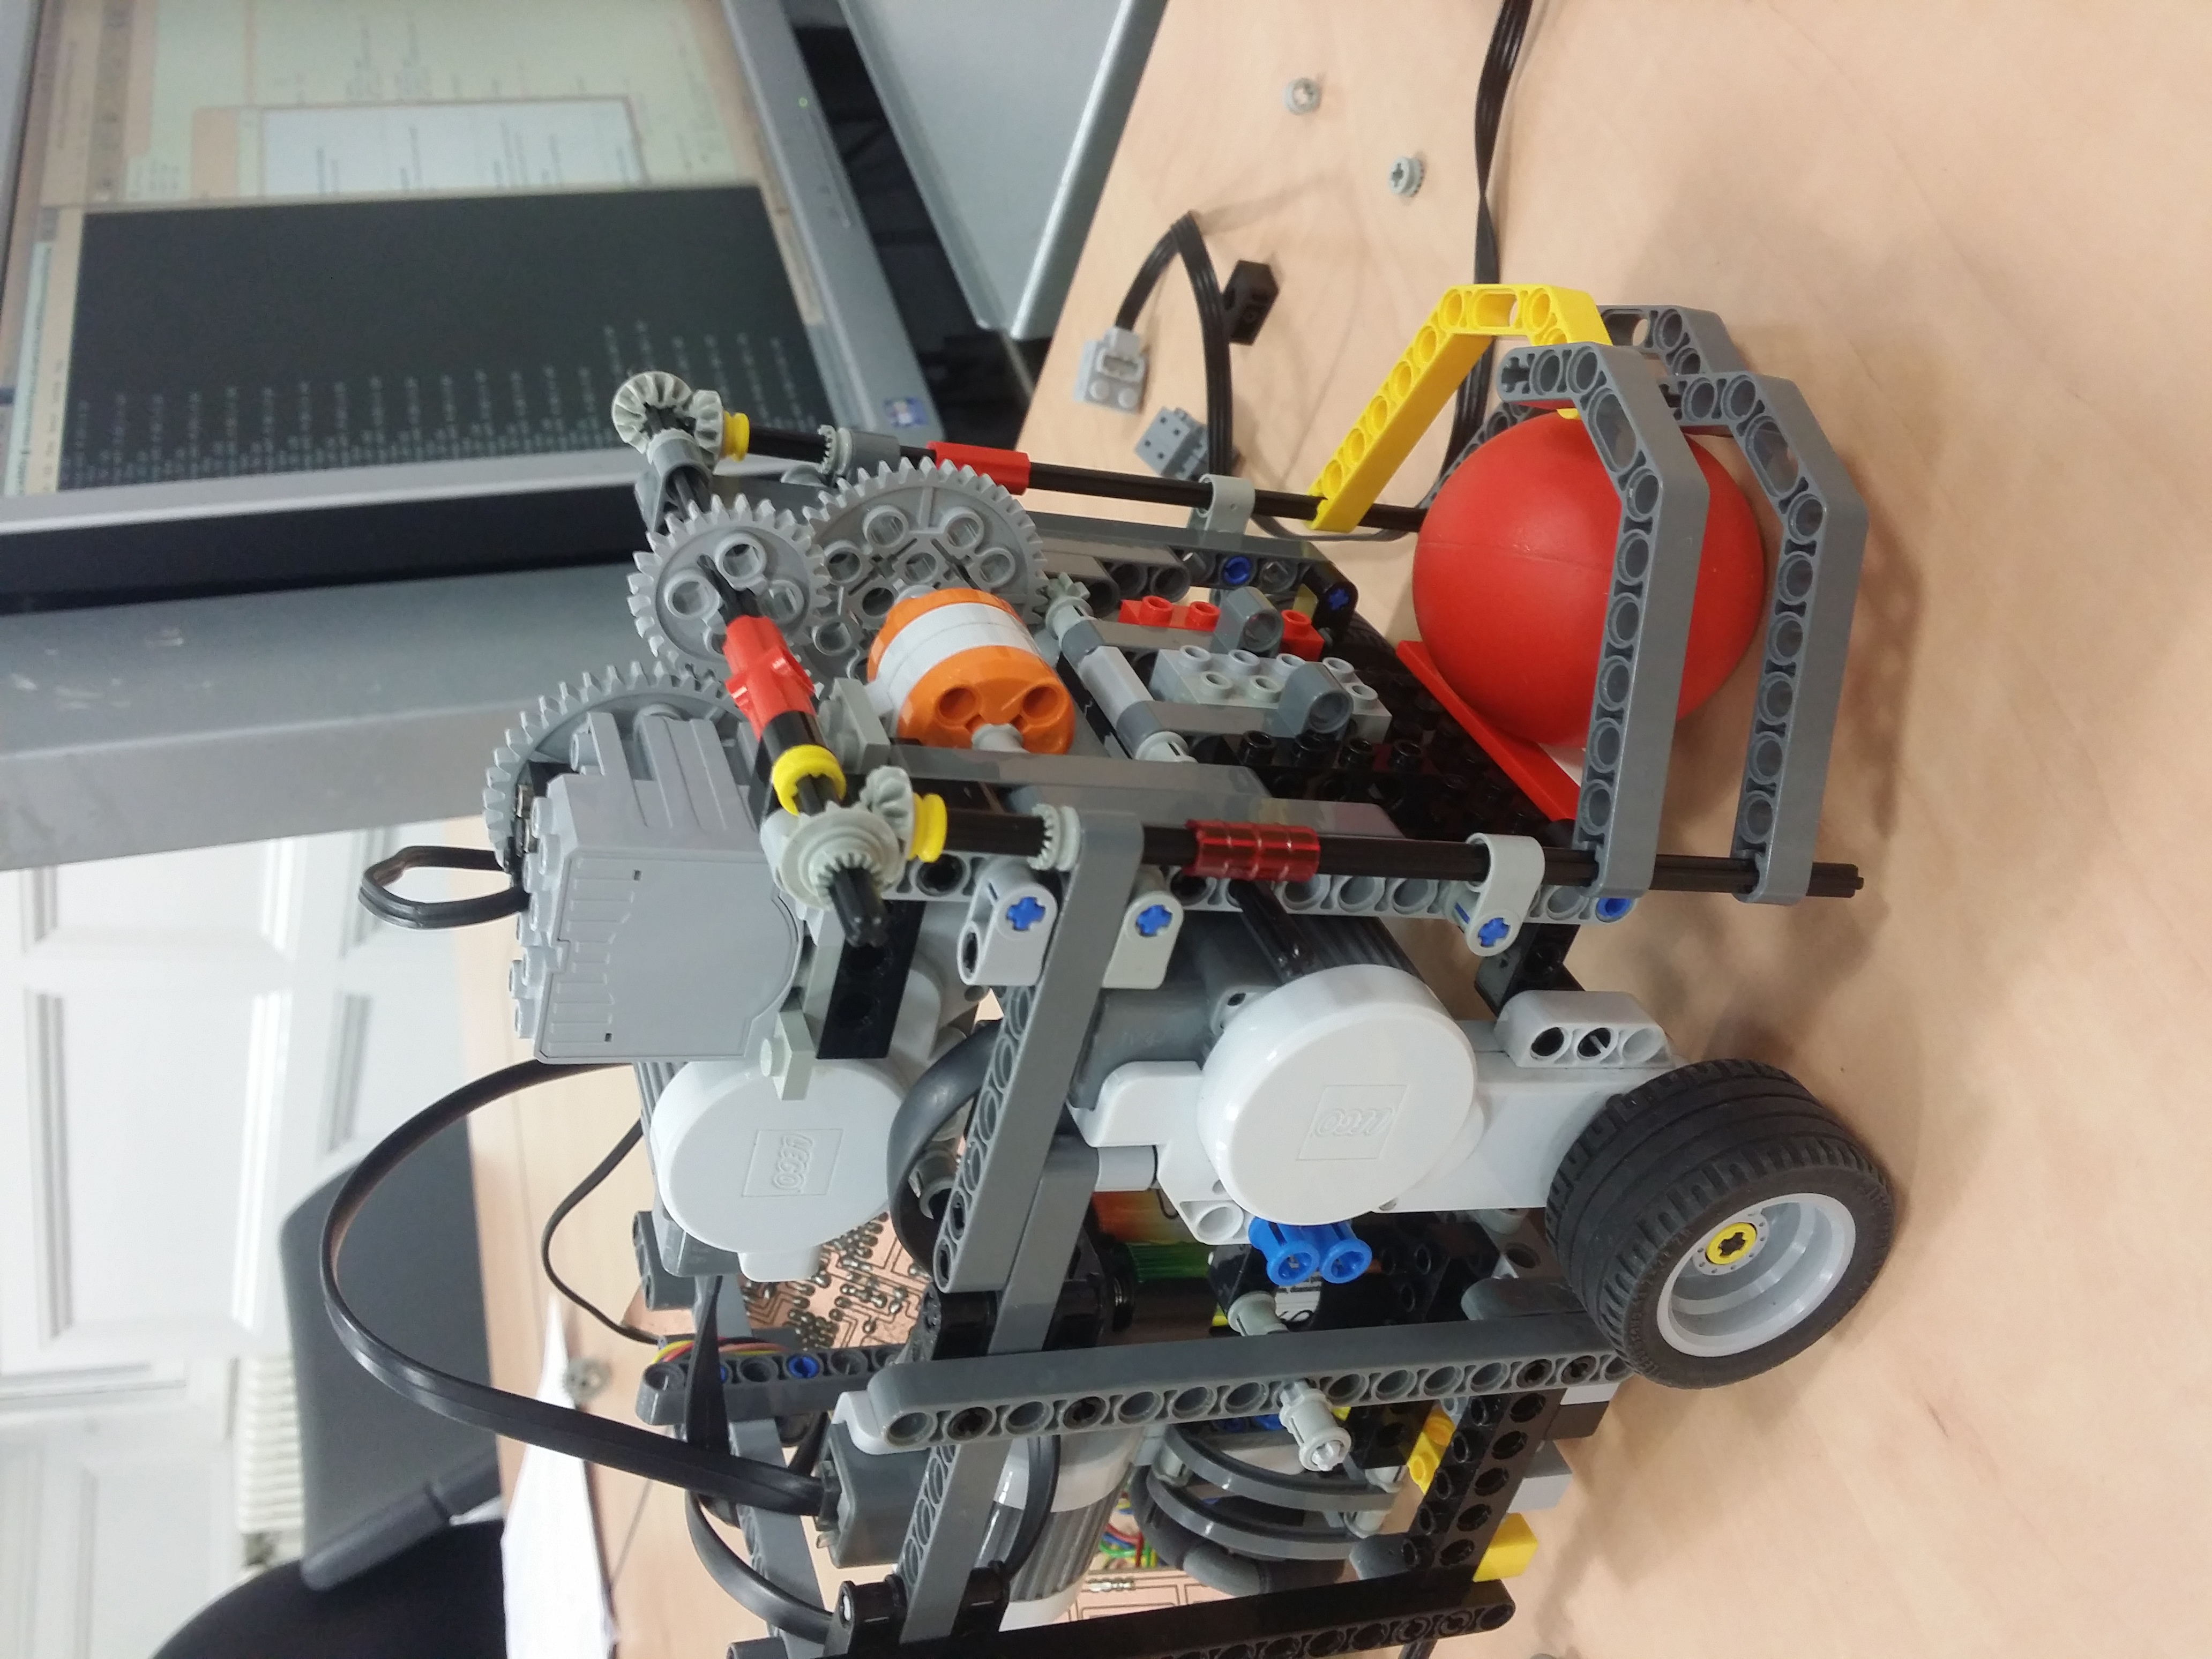
\includegraphics[scale=.065,angle=-90]{robot2.jpg}
		\caption{The third robot with the current grabber}
		\label{fig:robot2}
	\end{minipage}
\end{figure}


\section{Hardware}

The initial robot had four holonomic wheels. The current design has two main
driving wheels and one holonomic wheel placed sideways at the back which allows
the robot to turn as well as does not cause problems moving backwards and
forwards due to its holonomic property.

Even though the idea of the kicker that uses elastics was appealing as this made
the kick more powerful, it was almost impossible to predict the distance the
ball will travel.
Because of that the new design that was used for the first milestone has a
kicker that is powered by an NXT motor with gears. The kicker operates by going backwards inside the robot from the starting low position and then kicks
forwards and touches the ball.


\section{Documentation of the code}

\subsection{Communications}

The communication interface between the Arduino and PC is low level, that is,
the PC decides and specifies the individual motor numbers and rotary encoder
values or time durations for which they are going to be powered. Then the robot
turns the motors on, sets the timeouts to stop them, and notifies the PC about
finishing starting the motors as seen in Figure \ref{fig:code1}.

\begin{figure}
    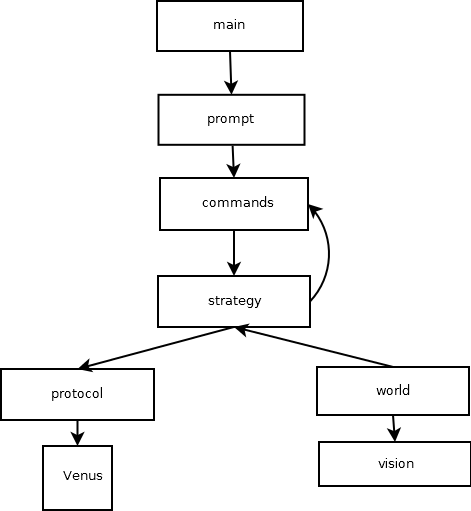
\includegraphics[scale=.7]{Diagram2}
    \caption{High level diagram of the system structure}
    \label{fig:code1}
\end{figure}

The messages are human-readable, newline-terminated and tokens inside them are
separated by spaces. The following messages are available:

\begin{tabular}{ | l | l | }
    \hline
    Rotate the motors for $n$ ms &
    \texttt{M <n> <motorCount> <no> <power>...} \\ \hline
    Rotate the motors until $n$ rotary value &
    \texttt{R <n> <motorCount> <no> <power>...} \\ \hline
    Stop all motors &
    \texttt{S} \\ \hline
    Transfer a byte to I2C bus &
    \texttt{T <byteInDecimalASCII>} \\ \hline
\end{tabular}

The specified motor power can be negative, in which case it means backwards
direction.

\subsection{Arduino}

Arduino code uses \textit{SDPArduino} library to interact with the motors.
It also uses \textit{SerialCommand} library to buffer and tokenize the
commands received over the serial link. As seen before, there are two methods to
specify when to stop the motor: either time value or rotary encoder value.
In the case of time value a timeout is set to stop each single motor using
\textit{setTimeout} from the \textit{SimpleTimer} library.
In the case of rotary encoder value \textit{setInterval} is used which calls
a callback that queries the rotary encoder board each 30 ms and stops the motors
that reached the target rotary encoder value. These approaches using timers
allows the robot to receive commands asynchronously, that is, a command is not
blocking during its execution and the PC software could, for example, decide
to engage the kicker while the robot is in motion.

\subsection{PC}

The PC currently provides a simple command line interface mapping higher level
commands such as \texttt{f 100} meaning 'go forwards 100 meters' to
communication messages. They are described in detail in the user guide.

\subsection{Vision}

TBD

\subsection{Planning}

TBD

\subsection{Strategy}

TBD

\section{Sensors}
\subsection{Rotary encoder board}

Each NXT motor is connected to the rotary encoder board. This way the
information about how many rotations the motor performed since the last query
is available for the Arduino code. Every 30 ms we query the board and
check whether we have reached the target value. After the rotary value becomes
greater or equal to the target value, the appropriate motor is stopped.

\end{document}
